\section{Phân tích OLAP và giao diện}\label{sec:olap}
\subsection{Định nghĩa KPI nhất quán theo grain}
Gọi $D$ là tập đơn delivered và $I(D)$ là các dòng hàng thuộc tập đó. Các thước đo dùng xuyên suốt các màn hình là:
\begin{align}
\text{Doanh thu hàng} &= \sum_{i\in I(D)} price_i, &
\text{Cước} &= \sum_{i\in I(D)} freight_i,\\
\text{Thanh toán} &= \sum_{o\in D,\,payment_o\ne NULL} payment_o,\\
\mathrm{AOV} &= \frac{\text{Thanh toán}}{\#\{o\in D: payment_o\ne NULL\}}.
\end{align}
Số đơn và số dòng hàng là hai đại lượng khác nhau. Khi thống kê khách, dùng \code{customer_unique_id}, không đếm \code{customer_id}. Tỷ lệ mua lại bằng số khách có ít nhất hai đơn delivered chia tổng số khách có đơn delivered. Thanh toán chỉ cộng ở grain đơn; ví dụ truy vấn dưới đây lấy từ trang Tổng quan:
\begin{lstlisting}[language=SQL]
SELECT count(*) AS orders,
       count(total_payment_value) AS paid_orders,
       sum(total_payment_value) AS payment,
       avg(total_payment_value) AS aov
FROM dw.fact_customer_order
WHERE order_status = 'delivered';
\end{lstlisting}
Các thước đo đếm riêng biệt (số đơn, số khách) không cộng được xuyên danh mục, seller hay bang vì một đơn có thể chứa nhiều danh mục hoặc seller; AOV và tỷ lệ luôn tính lại từ tử số và mẫu số.

\subsection{Các thao tác OLAP theo từng màn hình}
Phần này mô tả những gì người dùng thực hiện được trên giao diện; mỗi thao tác là một lời gọi API riêng đến kho.

\begin{table}[H]\centering\small\renewcommand{\arraystretch}{1.15}
\begin{tabularx}{\linewidth}{p{2.3cm}YY}
\toprule Màn hình & Thao tác OLAP & Cách thực hiện trên giao diện\\\midrule
Tổng quan & Bốn thẻ KPI; xu hướng tháng; top danh mục & Doanh thu hàng, giá trị đơn trung bình, số khách kèm tỷ lệ mua lại, cước kèm tỷ lệ so với doanh thu hàng.\\
Thời gian & Drill-down / roll-up, slice, dice, pivot & Bộ lọc phân cấp Năm $\rightarrow$ Quý $\rightarrow$ Tháng $\rightarrow$ Ngày; nhấn cột để đi xuống, nút lên để gộp lại; chế độ nhiều năm (dice) và chế độ Tháng $\times$ Năm (pivot).\\
Khu vực & Drill-down, slice & Bang $\rightarrow$ thành phố; chọn bang thì danh mục lọc theo bang; slice theo năm, quý.\\
Người bán & Xếp hạng, slice, dice & Top 5/10/20 người bán theo danh mục, bang, kỳ; ``khối'' người bán $\times$ danh mục $\times$ bang.\\
Khách hàng & Drill-down, dice, ma trận, xếp hạng & Ba chiều: nhóm khách, địa lý, trạng thái đơn; dice theo nhiều bang và khoảng năm; ma trận bang $\times$ năm; top khách theo bang.\\
\bottomrule\end{tabularx}
\caption{Thao tác OLAP theo màn hình}
\end{table}

Màn Tổng quan (hình~\ref{fig:ui-overview}) gom bốn thẻ KPI và bốn biểu đồ thu nhỏ, mỗi biểu đồ có nút mở sang màn chi tiết tương ứng. Biểu đồ thời gian ở đây chỉ hiện doanh thu theo tháng; tăng trưởng được xem ở màn Thời gian.

\begin{figure}[H]\centering
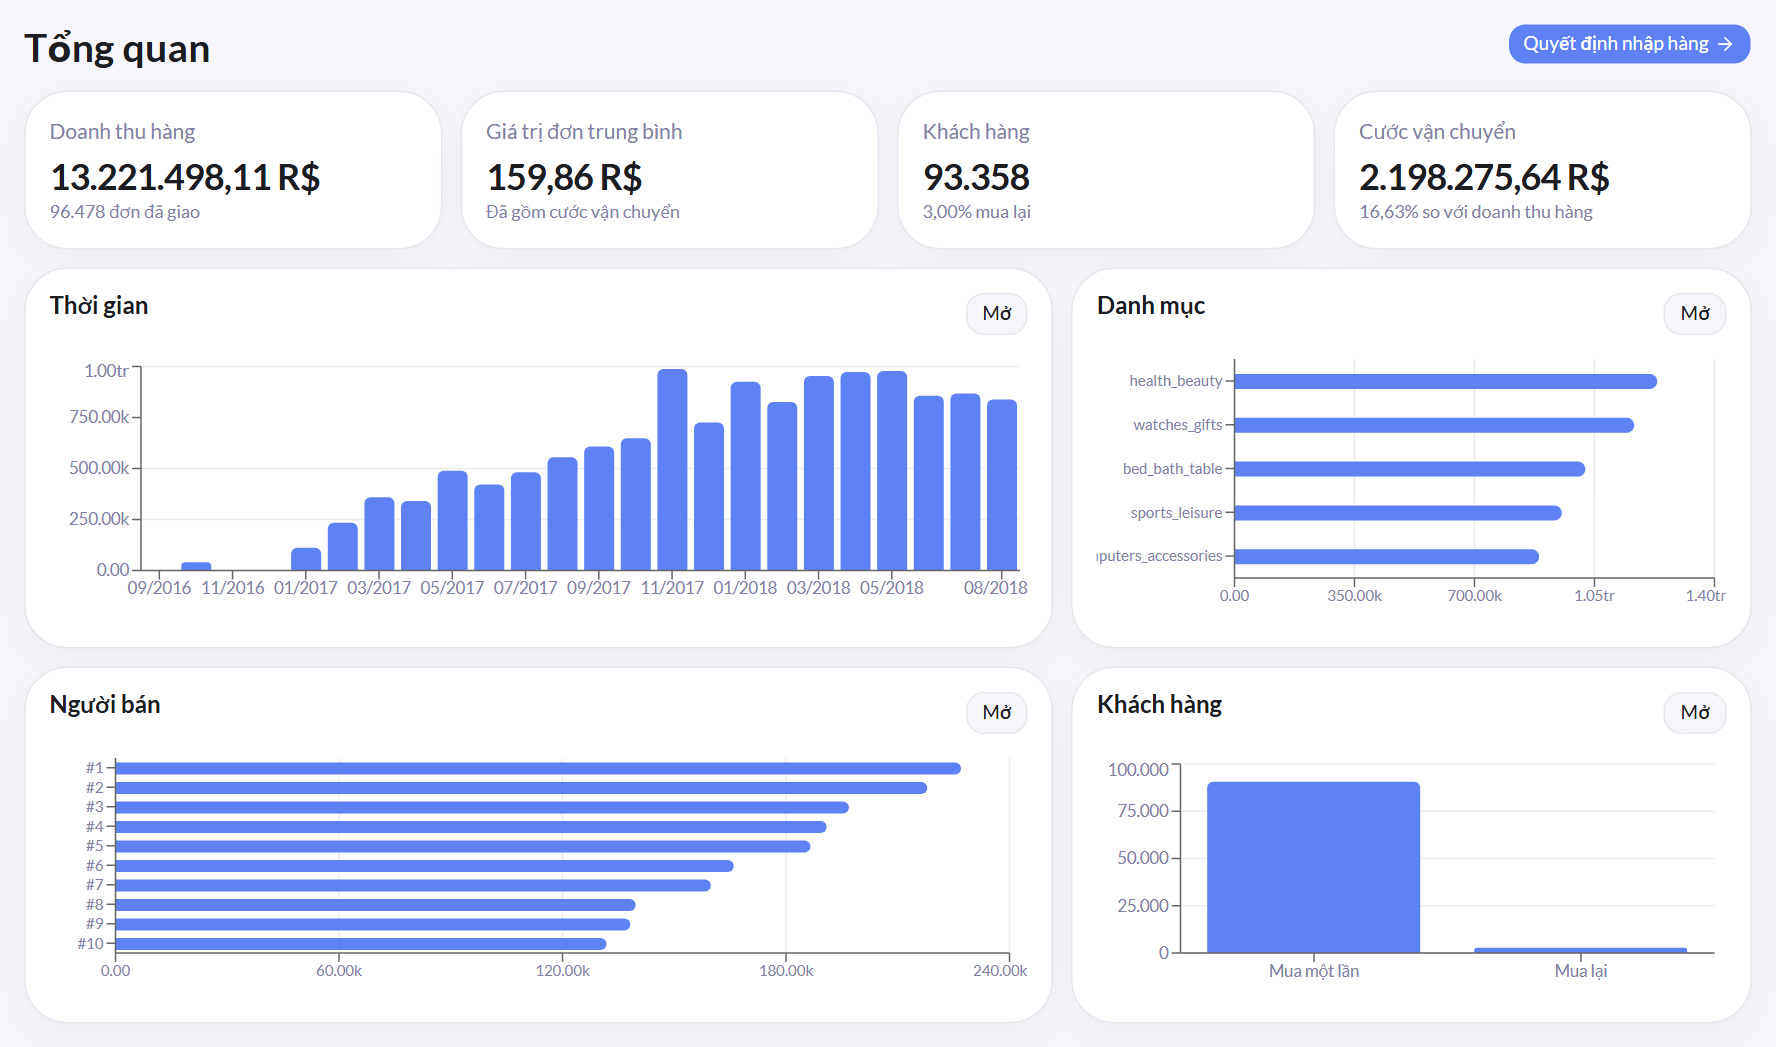
\includegraphics[width=\linewidth,height=0.42\textheight,keepaspectratio]{assets/ui_overview.png}
\caption{Màn Tổng quan}\label{fig:ui-overview}
\end{figure}


\subsubsection*{Màn Thời gian}
Chọn một trong ba thước đo: Doanh thu, Phí vận chuyển, Số lượng sản phẩm. Ở cấp năm và quý, bảng kèm tăng trưởng YoY và QoQ cùng kỳ, nghĩa là chỉ so các tháng có dữ liệu ở cả hai kỳ. Cách này cần thiết vì dữ liệu delivered chỉ phủ từ 09/2016 đến 08/2018 và thiếu 11/2016; chia tổng cả năm cho tổng cả năm trước sẽ trộn tăng trưởng thật với số tháng chênh lệch. Ví dụ 2018 (tháng 1--8) so với cùng các tháng của 2017 tăng +141,13\%, trong khi so với cả 12 tháng 2017 chỉ ra +21,05\%. Bảng cũng ghi số tháng có dữ liệu và số tháng dùng để so sánh. Ở cấp tháng, bảng hiển thị MoM; LAG được tính trên toàn chuỗi trước khi lọc nên tháng đầu của một kỳ vẫn có giá trị so sánh.

Ba loại tăng trưởng này dùng chung một quy tắc để loại các tháng gần như trống. Hai tháng 09/2016 (134,97 R\$) và 12/2016 (10,90 R\$) chỉ bằng 0,00--0,06\% trung vị nên không được dùng làm mốc so sánh. Một tháng bị coi là quá thưa khi nhỏ hơn 1\% trung vị các tháng có dữ liệu của cùng thước đo. MoM để trống khi tháng trước quá thưa, nên 10/2016 và 01/2017 không có MoM thay vì những con số vô nghĩa như +1.025.573\% làm trục biểu đồ giãn ra. Với QoQ và YoY, một cặp tháng cùng vị trí ở hai kỳ chỉ được đem so khi cả hai tháng đều đạt ngưỡng. Vì vậy Q1/2017 chỉ so 01/2017 với 10/2016 và tăng 177,24\% thay vì 1.067,68\%, còn Q4/2016 không còn cặp nào để so nên để trống.

Riêng YoY còn một điều kiện nữa là phải có ít nhất 3 cặp tháng hợp lệ, nếu không thì để trống. Lý do là tăng trưởng của cả một năm mà chỉ dựa trên một hoặc hai tháng thì không còn là so sánh theo năm, mà chỉ là tăng trưởng của vài tháng lẻ. Trên dữ liệu thật, YoY của 2017 so với 2016 chỉ có một cặp hợp lệ (10/2017 với 10/2016, tăng khoảng +1.507\%, một con số lớn vì mốc so sánh còn rất nhỏ) nên để trống, thay vì +4.796\% khi ghép cả các tháng gần như trống. YoY của 2018 có 8 cặp (tháng 1--8) nên vẫn là +141,13\%. Mức 3 tháng tương đương một quý, đơn vị nhỏ nhất của các so sánh theo kỳ trên màn này. Cột số tháng so cùng kỳ cho người đọc thấy mỗi kỳ dựa trên bao nhiêu tháng; QoQ không đặt điều kiện này nên Q1/2017 vẫn hiển thị kèm số 1.

Ngưỡng được đặt theo trung vị vì trung vị không bị kéo lệch bởi chính các tháng gần như trống ở đầu chuỗi, tháng Black Friday 11/2017 hay đà tăng mạnh từ 2017 sang 2018, trong khi trung bình chịu ảnh hưởng của các giá trị này. Ngưỡng cũng là tỷ lệ so với trung vị của từng thước đo nên dùng chung được cho doanh thu, cước (R\$) và số món mà không cần đặt một ngưỡng tuyệt đối riêng cho mỗi đơn vị. Mức 1\% không nhạy vì tháng thật nhỏ nhất (10/2016) đã bằng khoảng 6,5\% trung vị, nên mọi ngưỡng từ 0,1\% đến 6\% cho cùng kết quả. Báo cáo không nâng ngưỡng lên khoảng 10\% chỉ để bỏ nốt tháng 10/2016, vì mức đó chỉ cách tháng 01/2017 (khoảng 17--19\% trung vị) chưa đến 3 lần và trông như chỉnh ngưỡng cho khớp một tháng; điều kiện số tháng tối thiểu của YoY có lý do riêng nên được dùng thay thế.

Chế độ nhiều năm (dice) gộp theo năm, quý, tháng hoặc ngày trong một khoảng năm, với bộ lọc quý, tháng và loại ngày (cuối tuần hay ngày thường). Chế độ pivot và nút ma trận hiển thị biểu đồ cùng bảng Tháng $\times$ Năm. Tháng không có giao dịch để trống thay vì ghi 0, để không tạo mức giảm giả.

Hình~\ref{fig:ui-time} là màn Thời gian ở cấp năm, bảng bên dưới cho thấy tăng trưởng cùng kỳ cùng số tháng dùng để so sánh; hình~\ref{fig:ui-pivot} là chế độ pivot Tháng $\times$ Năm, gồm biểu đồ cột theo năm và bảng ma trận tương ứng.

\begin{figure}[H]\centering
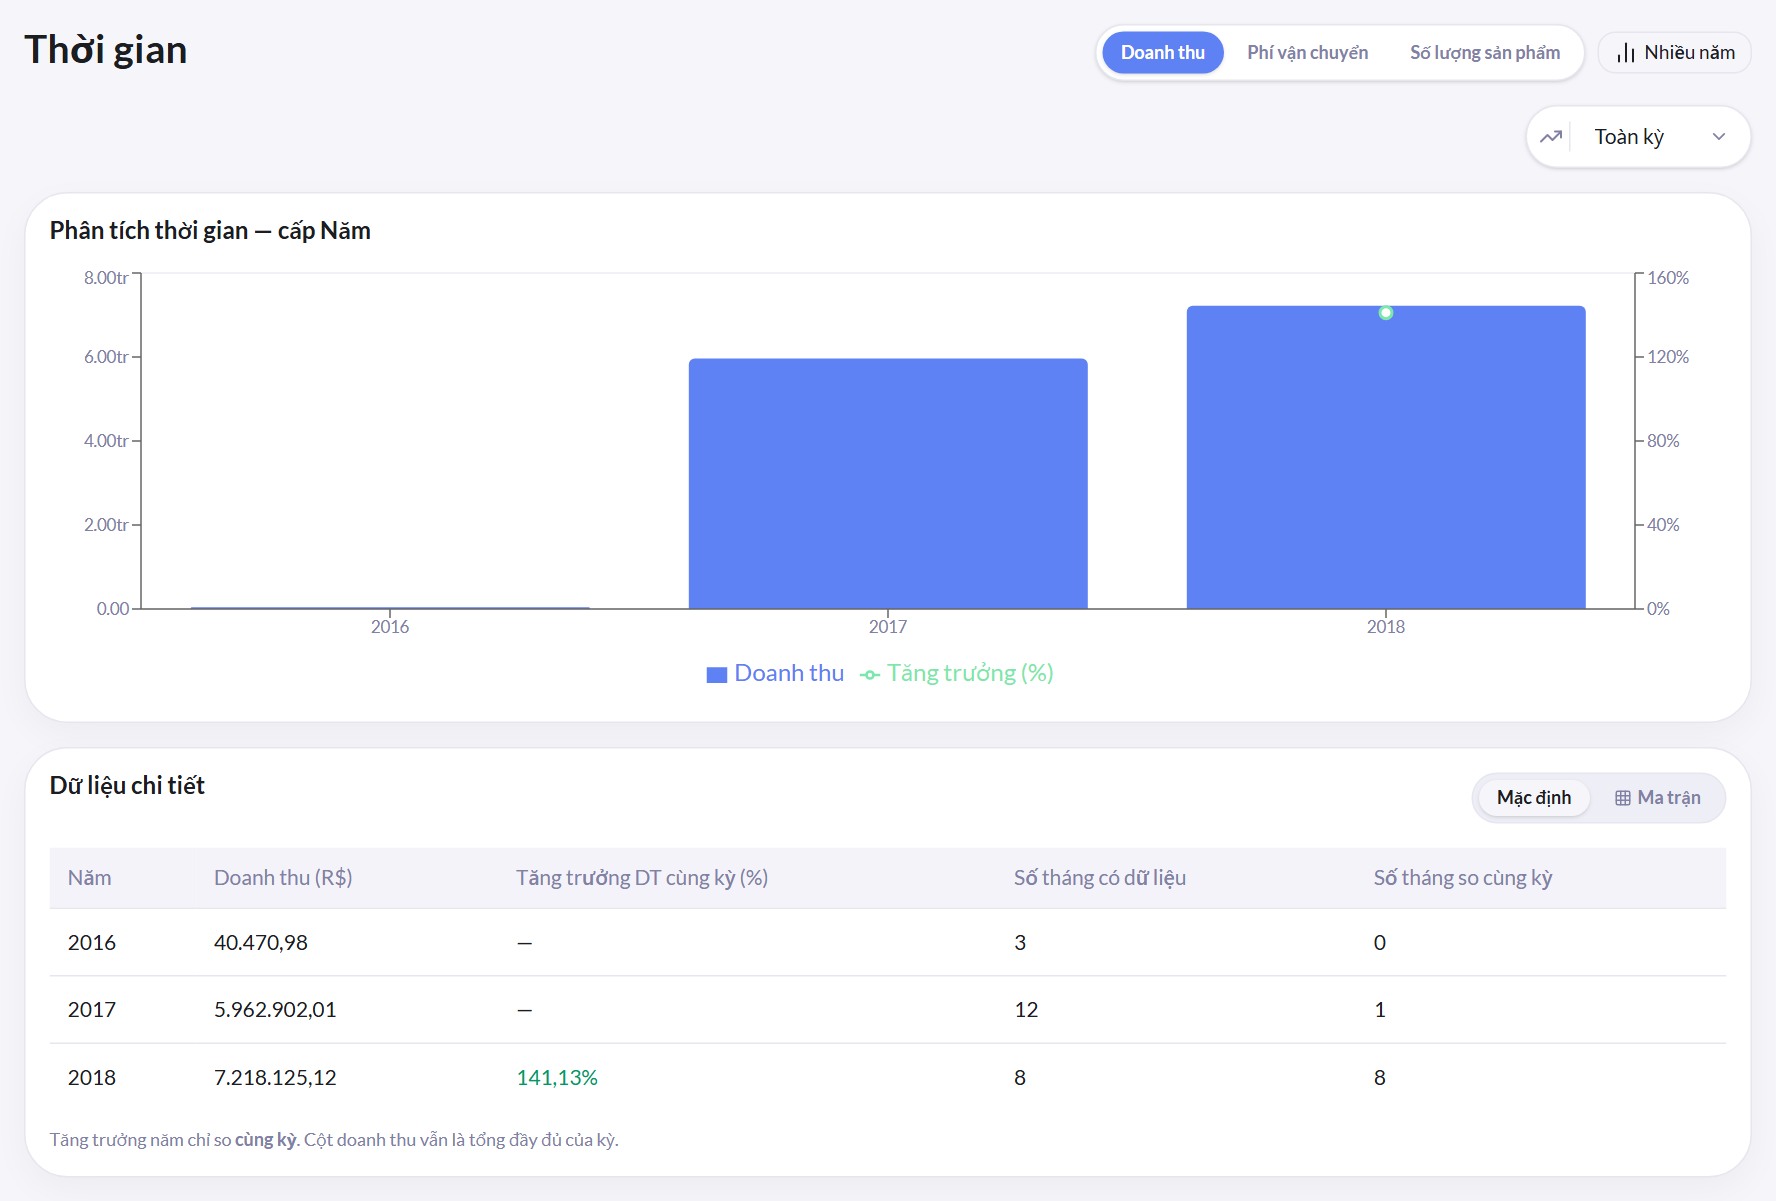
\includegraphics[width=\linewidth,height=0.42\textheight,keepaspectratio]{assets/ui_time.png}
\caption{Màn Thời gian ở cấp năm}\label{fig:ui-time}
\end{figure}

\begin{figure}[H]\centering
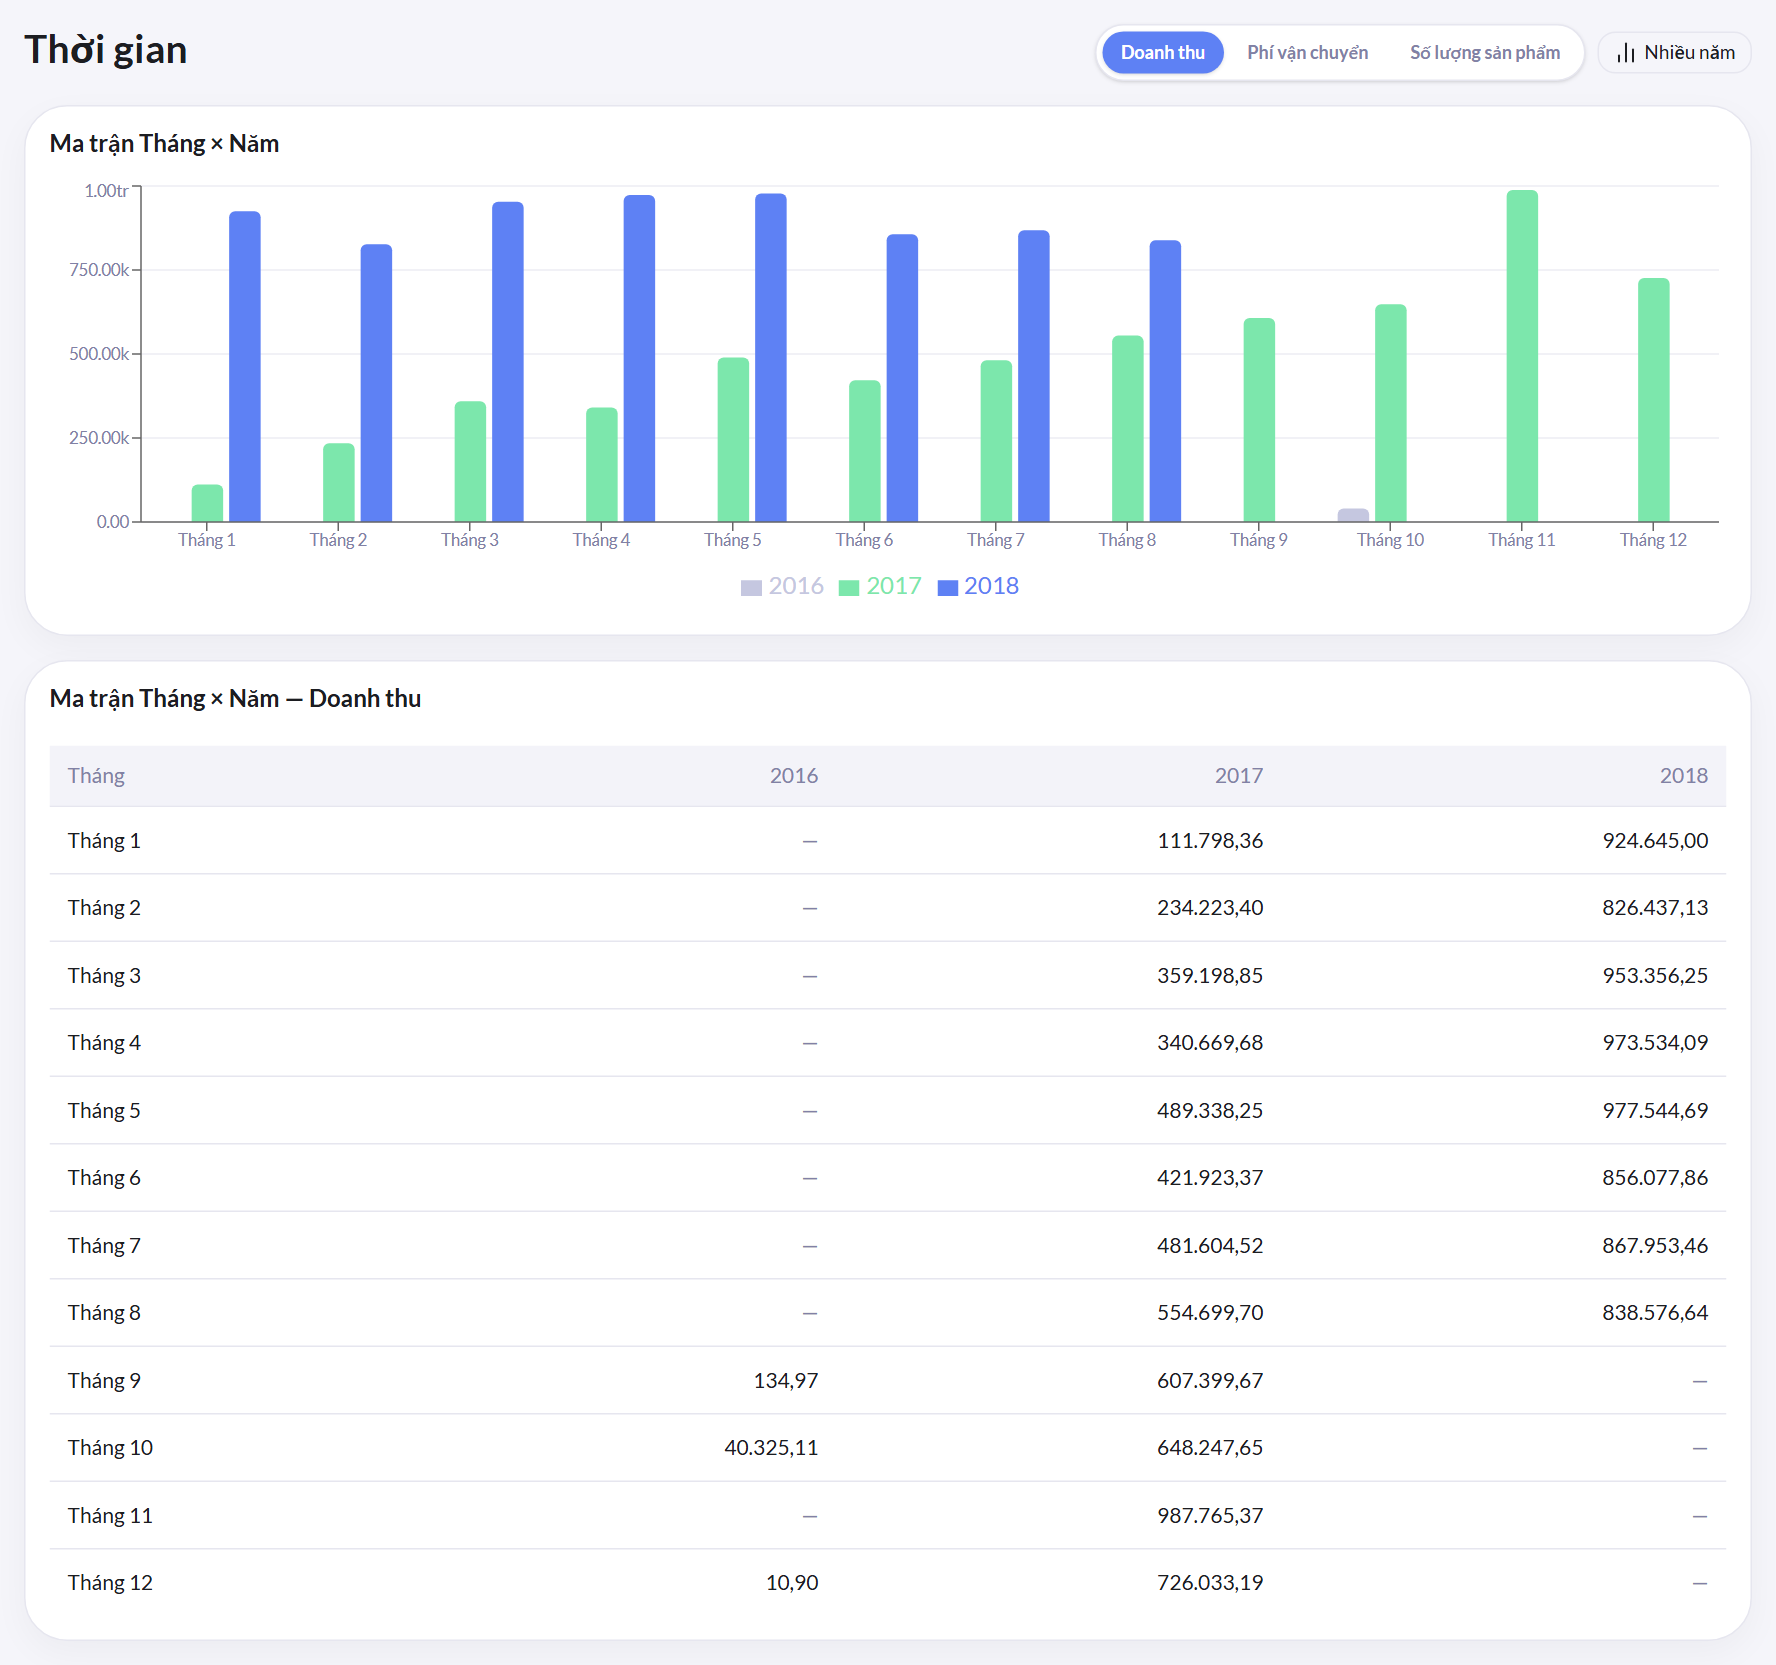
\includegraphics[width=\linewidth,height=0.5\textheight,keepaspectratio]{assets/ui_time_pivot.png}
\caption{Pivot Tháng $\times$ Năm}\label{fig:ui-pivot}
\end{figure}

\subsubsection*{Màn Khu vực và Người bán}
Màn Khu vực hiển thị doanh thu, cước, tỷ lệ cước/giá và số đơn; bảng bang chuyển sang thành phố của bang được chọn và danh mục được lọc theo bang. Bộ lọc năm và quý là thao tác slice. Màn Người bán xếp hạng top 5, 10 hoặc 20 người bán, lọc theo danh mục và bang khách; nút ``Xem khối'' dựng khối người bán $\times$ danh mục $\times$ bang cho nhiều danh mục và nhiều bang, với tổng theo bang và theo danh mục, và cho phép lấy một người bán, bang hoặc danh mục làm lát cắt. Địa lý trong cả hai màn là nơi khách đặt đơn, không phải nơi người bán.

Hình~\ref{fig:ui-geo} là màn Khu vực ở toàn kỳ, còn hình~\ref{fig:ui-cube} là khối người bán khi chọn ba danh mục health\_beauty, watches\_gifts, bed\_bath\_table và ba bang SP, RJ, MG.

\begin{figure}[H]\centering
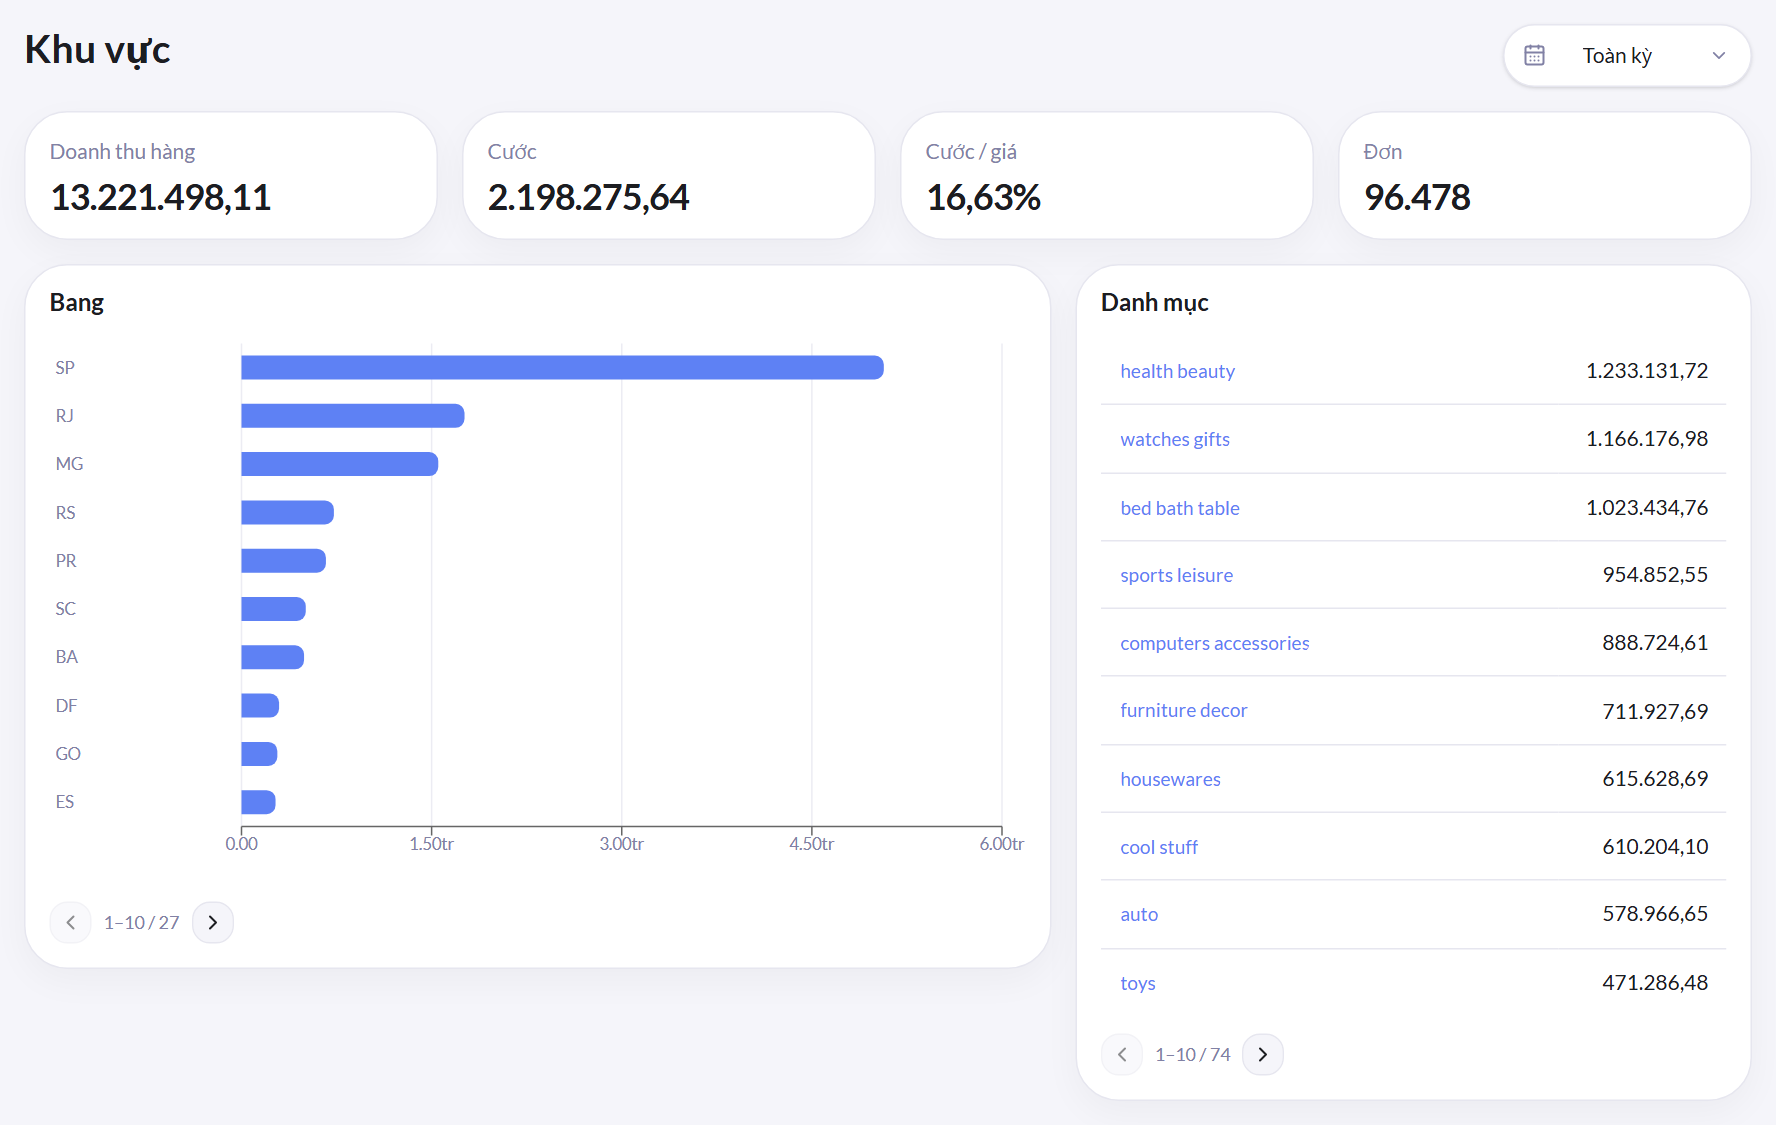
\includegraphics[width=\linewidth,height=0.42\textheight,keepaspectratio]{assets/ui_geo.png}
\caption{Màn Khu vực}\label{fig:ui-geo}
\end{figure}

\begin{figure}[H]\centering
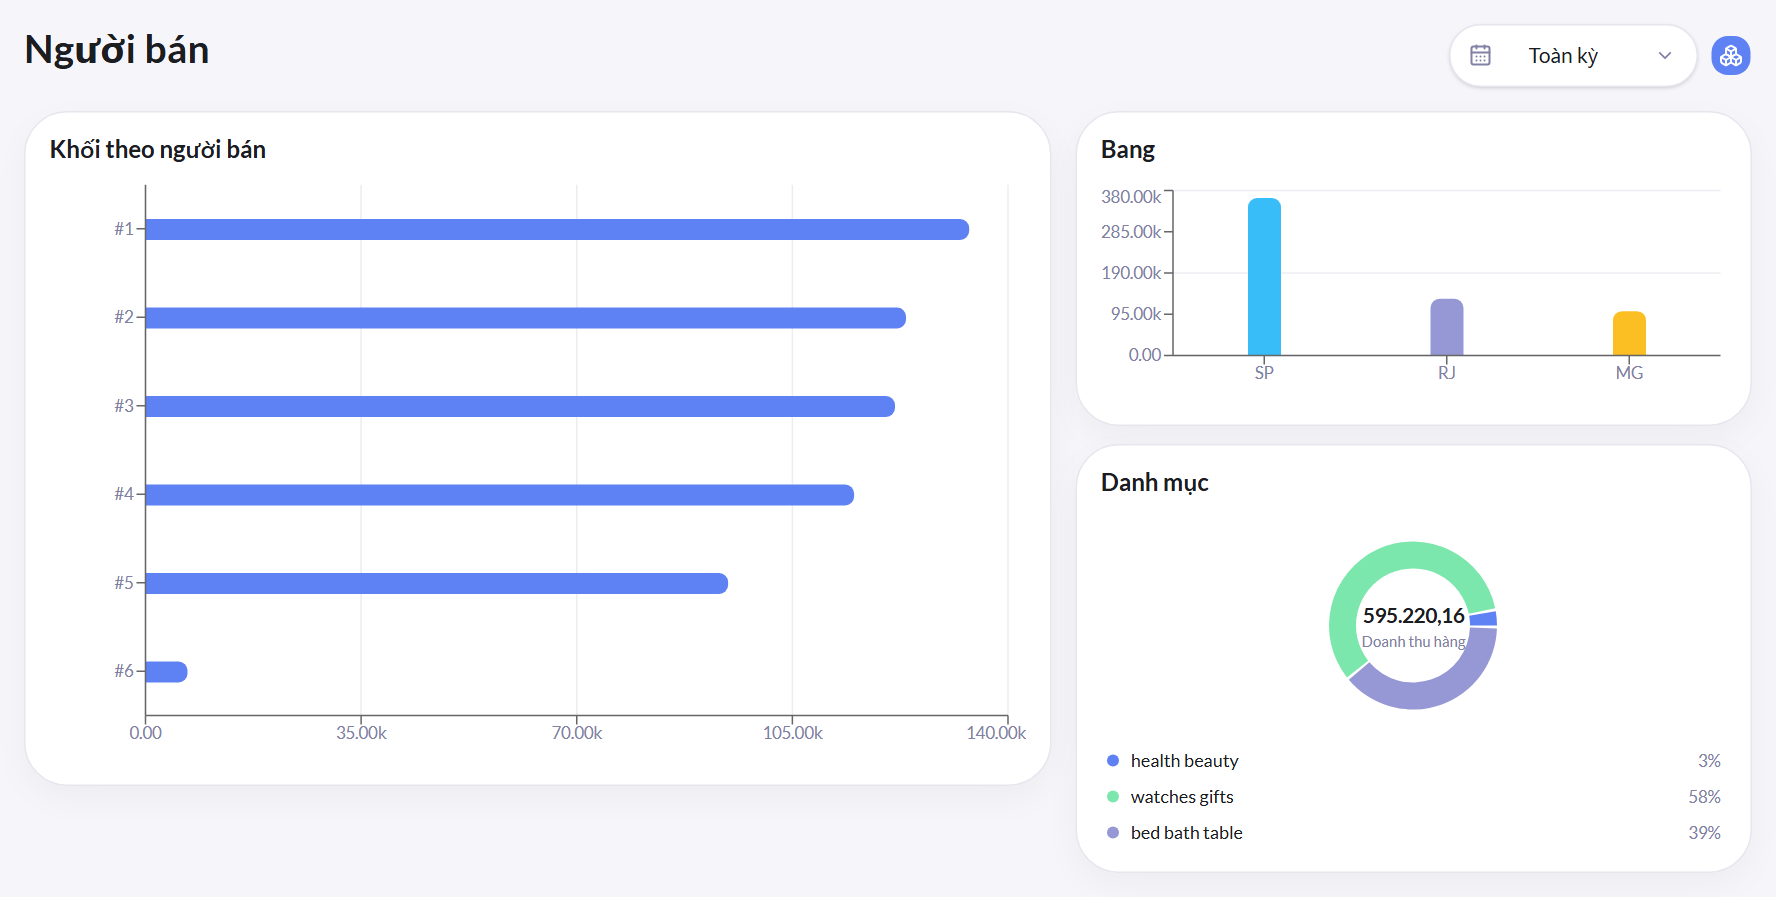
\includegraphics[width=\linewidth,height=0.42\textheight,keepaspectratio]{assets/ui_seller_cube.png}
\caption{Khối người bán $\times$ danh mục $\times$ bang}\label{fig:ui-cube}
\end{figure}

\subsubsection*{Màn Khách hàng}
Biểu đồ đổi giữa bốn thước đo: số khách, số đơn, thanh toán, AOV. Ba chiều drill-down gồm nhóm khách (mua một lần/mua lại), địa lý (bang $\rightarrow$ thành phố) và trạng thái đơn. Chế độ dice chọn nhiều bang và khoảng năm. Bảng chi tiết có thể đổi sang ma trận bang $\times$ năm; ngoài ra có bảng top 3 khách chi tiêu nhiều nhất mỗi bang kèm phân vị toàn quốc. Số khách riêng biệt không cộng xuyên bang hay năm; thành phố drill-down chỉ trả top 15 nên tổng hiển thị có thể nhỏ hơn tổng của bang.

Hình~\ref{fig:ui-customer} là màn Khách hàng theo nhóm mua một lần và mua lại, kèm bảng top 3 khách mỗi bang.

\begin{figure}[H]\centering
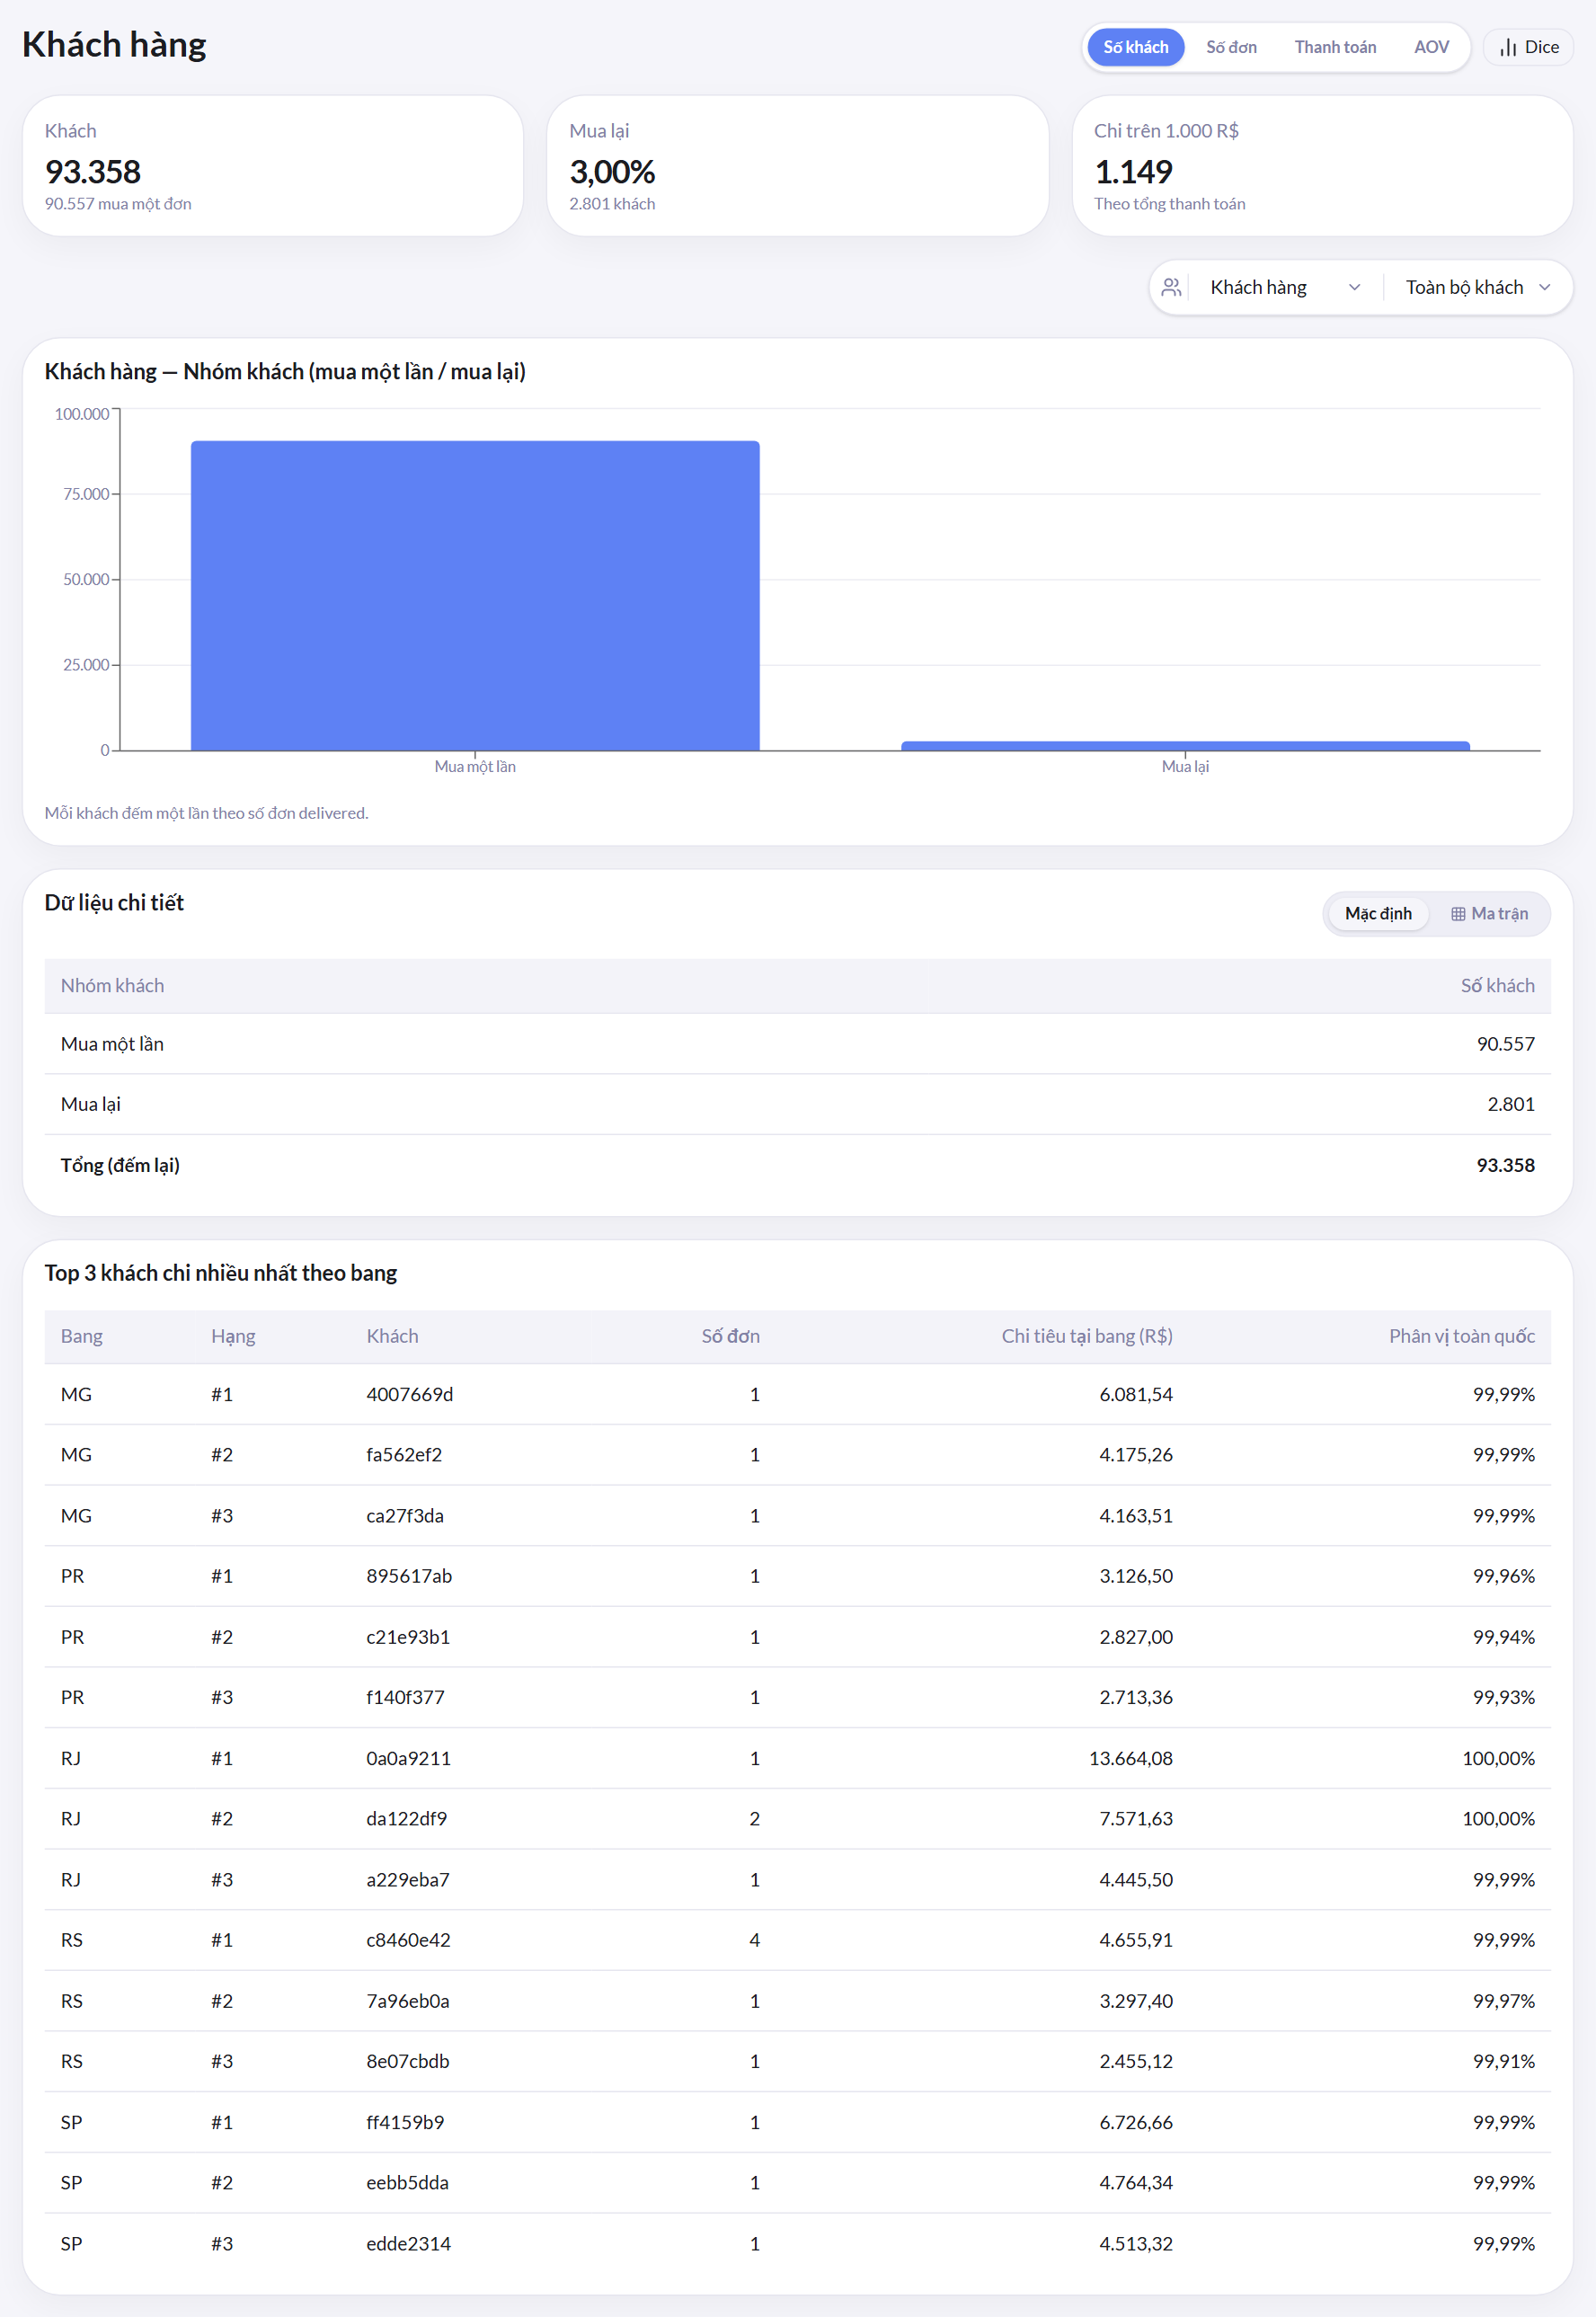
\includegraphics[width=\linewidth,height=0.62\textheight,keepaspectratio]{assets/ui_customer.png}
\caption{Màn Khách hàng}\label{fig:ui-customer}
\end{figure}

\subsection{API và công nghệ hiển thị}
Mỗi màn có nhóm API riêng (\code{/api/sales-time}, \code{/api/olap}, \code{/api/product-geo}, \code{/api/customer-payment}, \code{/api/overview}, \code{/api/dss}). Tên cột SQL lấy từ danh sách cho phép chứ không từ chuỗi truy vấn; giá trị lọc được tham số hóa (riêng năm, quý, tháng ở API Thời gian được ép kiểu số nguyên), tham số sai trả mã 400. Bộ lọc của bốn màn Thời gian, Khu vực, Người bán và Khách hàng được giữ trong URL để chia sẻ trạng thái màn hình, còn màn Người bán dùng lại API Khu vực.
